\subsection{Overview}
The device is composed of two distinct systems, the \textit{Computing Platform} and the \textit{Multirotor}, which work in tandem to capture aerial video, analyze it through hardware-accelerated processes, and convey the results of the analysis to the end-user. 

\begin{figure}[H]\label{hlpic}
    \centering
    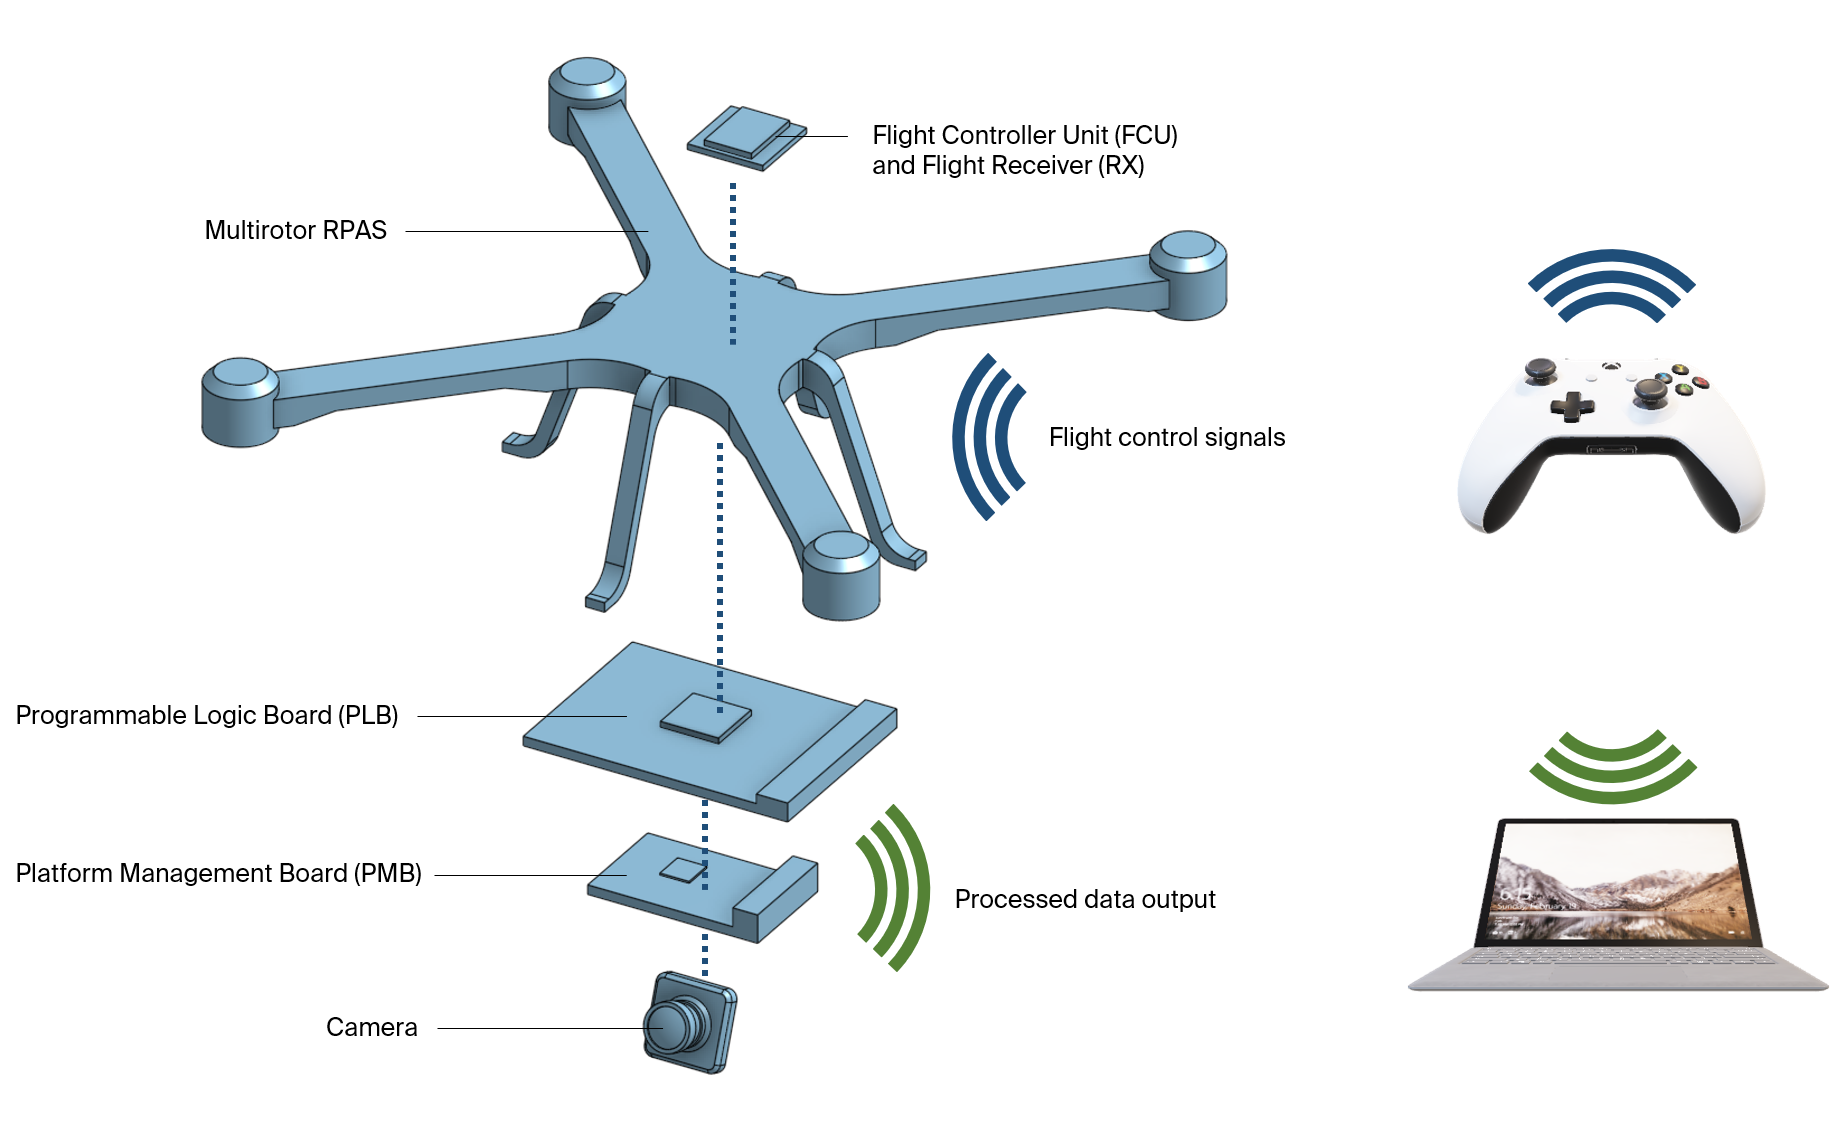
\includegraphics[width=\linewidth]{img/intpic.png}
\caption{High-Level System Integration with RPAS}
\end{figure}

\textbf{The \textit{Computing Platform}} is comprised of three processing platforms: the \textit{Platform Management Board} (PMB), the \textit{Programmable Logic Board} (PLB), and the \textit{Base Station}. The \textit{PMB} and \textit{PLB} are mounted to the multirotor, while the base station is a mobile device utilized by the user at ground-level.

The \textit{Platform Management Board} (a Raspberry Pi 4) is responsible for managing the majority of the aerial computations. This includes managing video acquisition, conveying data to and from the PLB to facilitate hardware accelerated machine learning tasks, and transmitting video and ML results to the base station over a WiFi connection.

The \textit{Programmable Logic Board} (a Digilent Zedboard), connected to the PMB via Ethernet, facilitates the hardware-acceleration functionalities of the device. It is comprised of a hard-processor (ARM Cortex A9) and an FPGA interfaced via an on-chip interconnect. The FPGA hosts the hardware acceleration unit, which is (currently) driven by the Zynq-7000 YoloV2 open-source accelerator\cite{yolov2accel}. As this device is intended to act as an experimental research platform, client may replace this with their own hardware accelerator implementation upon delivery.

The \textit{Base Station} (a consumer laptop) connects to the multirotor via WiFi, displaying live video and ML results as transmitted by the aerial computing components. In addition to conveying the video and its ML analytics, the base station also provides remote control of the computing system -- allowing the user to monitor system status and alter parameters of ongoing computations on-the-fly.

\textbf{The \textit{Multirotor}} is a quad-engine remote-piloted-aerial system, or multirotor/quadcopter RPAS for short.
The RPAS is propelled electrically using DC sources and motors, controlled by an onboard flight controller unit (FCU) that samples accelerometer data to make fine adjustments to the flight kinematics.
The RPAS is equipped with a receiver to enable flight control via standard radio-control (RC, 2.4 GHz) by a pilot.

The RPAS and computing platform are relatively independent as the computing platform provides its own power source. The two modules impose constraints on each other: the computing platform (including its power source) must be light and compact such that it can be lifted by the RPAS. 
Likewise, the RPAS must provide mounting mechanisms for the computing platform and provide clearance such that equipment is not damaged during flight operations.

\subsection{System Data Flow}

\begin{figure}[H]
\centering
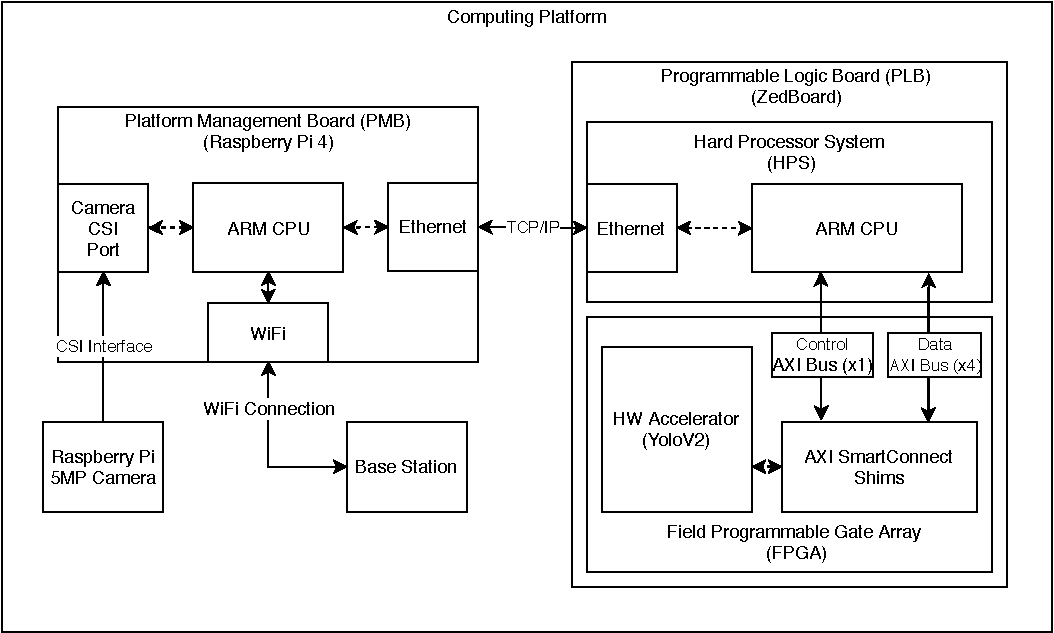
\includegraphics[width=15cm]{img/pc_diagram.pdf}
\caption{High-Level System Architecture}
\label{pcdiag}
\end{figure}

A step-by-step overview of data flow within the computing platform (refer to Figure \ref{pcdiag}) is as follows:
\begin{enumerate}
\item Video is captured using the 5MP Raspberry Pi Camera, and is transmitted to the PMB via a CSI interface
\item Video is decomposed into packets and sent to three locations:
\begin{enumerate}
\item Non-Volatile Memory, for future analysis, 
\item The PLB, via a TCP/IP ethernet link, to perform hardware-accelerated machine learning, and
\item The base station, via a TCP/IP WiFi link, to display to the end-user
\end{enumerate}
\item The ARM core on the PLB receives video packets from the PMB via the ethernet link, further processes it, and dispatches hardware acceleration requests to the FPGA portion via an AXI bus
\item The FPGA receives hardware acceleration requests (passing through an AXI shim to facilitate data transfer), passing it to the hardware accelerations core(s)
\item Upon completion, the hardware acceleration cores send data back to the ARM core, which itself transmits the resultant data back to the PMB via the Ethernet link
\item The machine learning results are transmitted over the WiFi link to the base station
\item The base station combines the video feed and machine learning results, displaying them on-screen
\end{enumerate}

Simultaneously, the user independently controls the operation of the multirotor through a standard radio controller, as described in Section \ref{multirotor}.